\documentclass{llncs}
\usepackage{amsmath, amssymb, fancyvrb, multirow, color, stmaryrd}
\usepackage{svg}
\usepackage{wrapfig}
\usepackage{graphicx}
\usepackage{fancyvrb}
\usepackage{hyperref}
\usepackage[]{algorithm2e}

\newcommand{\enforce}{\mathsf{enforce}}
\newcommand{\traj}{\mathsf{traj}}
\newcommand{\dReal}{\textsf{dReal}}
\newcommand{\dReach}{\textsf{dReach}}

%\usepackage{multirow}
\usepackage{amsmath,hyperref}
\hypersetup{
    colorlinks,%
    citecolor=blue,%
    filecolor=blue,%
    linkcolor=blue,%
    urlcolor=blue
}
\usepackage{amssymb,verbatim}
\usepackage{fix2col,listings,fancyvrb}
\usepackage{multicol}
\usepackage{graphicx,epsfig}
\usepackage{caption}
\usepackage{stmaryrd}
\usepackage{setspace}
\usepackage{ulem}
\usepackage{newlfont}
\usepackage{epsfig,graphics}
\usepackage{fancybox}
\usepackage{listings}
\usepackage{caption}
\usepackage{graphicx,epsfig}
\usepackage{caption}
\usepackage{makeidx}
\usepackage{algorithm}
\usepackage{algpseudocode}
\usepackage{listings}
\lstset{
  basicstyle=\ttfamily,
  breaklines=true,
  columns=fullflexible,
  escapeinside = ||,
  breakindent=0pt}
\makeindex

\usepackage{algorithm}
\usepackage{algpseudocode}
\usepackage{hyperref}
\hypersetup{
    colorlinks,%
    citecolor=blue,%
    filecolor=blue,%
    linkcolor=blue,%
    urlcolor=blue
}
\usepackage{multicol}
\usepackage{lipsum}

\newtheorem{theorem}{Theorem}
\newtheorem{proofoutline}[theorem]{Proof Outline}
\newtheorem{lemma}[theorem]{Lemma}
\newtheorem{claim}[theorem]{Claim}
\newtheorem{proposition}[theorem]{Proposition}
\newtheorem{corollary}[theorem]{Corollary}
\newtheorem{fact}[theorem]{Fact}
\newtheorem{definition}[theorem]{Definition}
\newtheorem{remark}[theorem]{Remark}
\newtheorem{conjecture}[theorem]{Conjecture}
\newtheorem{example}[theorem]{Example}
\newtheorem{notation}[theorem]{Notation}
\newtheorem{question}[theorem]{Question}



%\usepackage[ruled,lined,boxed,commentsnumbered,linesnumbered]{algorithm2e}

\setcounter{secnumdepth}{3}
\setcounter{tocdepth}{2}

\newcommand\bookepigraph[4]{
\vspace{1em}\hfill{}\begin{minipage}{#1}{\begin{spacing}{0.9}
\small\noindent\textit{#2}\end{spacing}
\vspace{1em}
\hfill{}{#3}\\

\vspace{-1em}\begin{flushright}{#4}\end{flushright}}\vspace{2em}
\end{minipage}}

\newcommand{\dom}{\mbox{dom}}

\newcommand\epigraph[3]{
\vspace{1em}\hfill{}\begin{minipage}{#1}{\begin{spacing}{0.9}
\small\noindent\textit{#2}\end{spacing}
\vspace{1em}
\hfill{}{#3}}\vspace{2em}
\end{minipage}}

\newcommand\anonymousepigraph[2]{
\vspace{1em}\hfill{}\begin{minipage}{#1}{\begin{spacing}{0.9}
\small\noindent\textit{#2}\end{spacing}}
\vspace{1em}
\end{minipage}}

\newcommand{\len}{\mathit{len}}
\newcommand{\poly}{\mathsf{poly}}
\newcommand{\N}{\mathbb{N}}
\newcommand{\R}{\mathbb{R}}
\newcommand{\D}{\mathbb{D}}
\newcommand{\cf}{\mathsf{CF}}
\newcommand{\be}{\mathsf{BE}}
\newcommand{\fe}{\mathbb{F}^{[\underline{e}, \overline{e}]}_{\beta,p}}
\newcommand{\rad}{\mathrm{rad}}


\newcommand{\flow}{\mathsf{flow}}
\newcommand{\jump}{\mathsf{jump}}
\newcommand{\inv}{\mathsf{inv}}
\newcommand{\init}{\mathsf{init}}
\newcommand{\guard}{\mathsf{guard}}
\newcommand{\reset}{\mathsf{reset}}
\newcommand{\reach}{\mathsf{Reach}}
\newcommand{\unsafe}{\mathsf{unsafe}}

\newcommand{\safe}{\mathsf{safe}}
\newcommand{\p}{\mathsf{P}}
\newcommand{\np}{\mathsf{NP}}
%\newcommand{\dom}{\mathrm{dom}}


\newcommand\tupleof[1]{\left\langle #1 \right\rangle}
\newcommand\vI{\vec{I}}
\newcommand\va{\vec{a}}
\newcommand\vb{\vec{b}}
\newcommand\vc{\vec{c}}
\newcommand\vd{\vec{d}}
\newcommand\ve{\vec{e}}
\newcommand\vl{\vec{l}}
\newcommand\vu{\vec{u}}
\newcommand\vx{\vec{x}}
\newcommand\vy{\vec{y}}
\newcommand\trp[1]{#1^{{}^{\mbox{\sc{t}}}}}
\newcommand{\lrf}{\mathcal{L}_{\mathbb{R}_{\mathcal{F}}}}
%\usepackage{wrapfigure}

%\doublespacing


\title{\dReach{}: $\delta$-Complete Analysis Tool for Bounded Reachability of Hybrid Systems}

\begin{document}


\mainmatter  % start of an individual contribution

\author{Soonho Kong, Sicun Gao, Wei Chen, and Edmund Clarke}

\authorrunning{S. Kong, S. Gao, W. Chen,  E. Clarke}
\institute{Computer Science Department, Carnegie Mellon University, USA}
\maketitle

\abstract{dReach encodes reachability problems of hybrid systems to
  first-order formulas over real numbers. The formulas are solved by
  delta-complete decision procedures in the SMT solver dReal. In this
  way, dReach is able to handle a wide range of highly nonlinear
  hybrid systems. Experiments have shown promising results on many
  nonlinear benchmarks that are not solvable by other existing tools.}

% Tool demonstration papers focus on the usage aspects of tools. As with
% regular tool papers, authors are strongly encouraged to make their
% tools publicly available, preferably on the web. Theoretical
% foundations and experimental evaluation are not required, however, a
% motivation as to why the tool is interesting and significant should be
% provided. Tool demonstration papers can have a maximum of 6 pages.
% They should have an appendix of up to 6 additional pages with details
% on the actual demonstration.

% http://www.etaps.org/index.php/2014/tacas/accepted-papers
% - http://costa.ls.fi.upm.es/papers/costa/AlbertAFGGMPR14.pdf
% - http://maude.sip.ucm.es/~adrian/files/tacas14.pdf
% - http://www.cs.vu.nl/~wanf/pubs/cif3.pdf
% - http://www.loria.fr/~chevalvi/files/Cheval-tacas14.pdf
% - http://www.sci.unich.it/~fioravan/papers/2014-DFPP-TACAS14.pdf

\section{Introduction}\label{sec:intro}

% Need a paragrapgh or two to explain why the tool is interesting and
% significant should be provided.

\dReach{} is a bounded model checker for hybrid systems. It encodes
bounded reachability problems of hybrid systems as first-order
formulas over the real numbers, and solves them using
$\delta$-decision procedures in the SMT solver \dReal{}. \dReach{} is
able to handle a wide range of highly nonlinear hybrid systems. It has
scaled well on various realistic nonlinear models from biomedical and
robotics applications~\cite{}.

It is well-known that the standard bounded reachability problems for
simple hybrid systems are already highly
undecidable~\cite{DBLP:conf/rex/AlurD91,DBLP:conf/hybrid/AlurCHH92}. In
previous work~\cite{}, we have defined the notion of
$\delta$-reachability problem of hybrid systems. In this new
framework, we have shown that bounded $\delta$-reachability is
decidable for a wide range of hybrid systems, with reasonable
complexity bounds~\cite{}. We give a brief review of the framework in
Section~\ref{sec:delta-reachability}.

Realistic hybrid systems involves nonlinear ODEs with transcendental
functions. \dReach{} allows users to specify a hybrid system in a
nonlinear signature as it is without linearizing or overapproximating
it. Users can provide the tool with a numerical error bound $\delta$,
a bounded time horizon $[0, T]$, and a maximum number of mode switches
$k$ for the analysis. As a result of analysis, \dReach{} will return
either \textbf{$\delta$-sat} with a concrete counterexample, or
\textbf{unsat} which does not involve numerical errors. We also
provide a visualization for the $\delta$-sat case to help
understand the analysis result.
\begin{figure}[!t]
  \subfloat[An example of nonlinear hybrid system model: off-treatment
  mode of the prostate cancer treatement model~\cite{}\label{subfig-1:prostate}]{
    \includegraphics[width=0.48\textwidth]{images/prostatebw-mode2.pdf}
  }
  \hfill
  \subfloat[Visualization of a concrete counterexample generated from
  dReach for the prostate cancer treatment model.]{%
    \includegraphics[width=0.48\textwidth]{images/prostate}
  }
  \caption{An example of nonlinear hybrid system model: Prostate
    cancer model.}
  \label{fig:prostate-example}
\end{figure}
For instance, figure~\ref{fig:prostate-example} shows a part of a
prostate cancer treatment model that contains nonlinear ODEs and a
visualization of a generated concrete counterexample.

\paragraph{Related Work}
%reachable set computation tools: flow star, SpaceX, Phaver,
%theorem provers:
%similar tools: iSAT, RSolver -- emphasize on the nonlinearity that we can handle.

The paper is structured as follows.


%%% Local Variables:
%%% mode: latex
%%% TeX-master: "main"
%%% End:

\section{Preliminaries}

We give an overview of the floating point implementation of the sine function in the Embedded GNU C Library. We then briefly review SMT solving of nonlinear formulas over the reals and features of our solver dReal~\cite{}.

\subsection{Floating-Point Representations and Errors}

Floating point representations. 

It is well-known that floating point computation introduces errors. For basic arithmetic operations, the error can be estimated by the following formula. 

We use this formula to overapproximate the result of floating point arithmetic with real arithmetic. 

\subsection{Structure of the Implementation}

The basic idea of evaluating the sine function is, naturally, to combine the periodic nature of the function and estimate the value with Taylor series. For each input number, the routine checks its position with respect to multiples of $\pi/4$, and then evaluate the value with appropriate Taylor expansion. 

The implementation of the sine function has the following structure. 
\begin{verbatim}
Give a simplified skeleton
\end{verbatim}

We should highlight the bit-level operations and table look up in the formula. 

\subsection{SMT over the Reals}


SMT formulas over the real numbers are very hard to solve when nonlinear functions are involved. 
We let $\mathcal{F}$ denote a set of continuous real functions. $\mathcal{L}_{\mathcal{F}}$ denotes the first-order signature and $\mathbb{R}_{\mathcal{F}}$ is the standard structure $\langle \mathbb{R}, \mathcal{F}\rangle$. We can then consider the SMT problem over $\mathbb{R}_{\mathcal{F}}$, namely, satisfiability of quantifier-free $\mathcal{L}_{\mathcal{F}}$-formulas over $\mathbb{R}_{\mathcal{F}}$. We consider formulas whose variables take values from bounded intervals. Because of this, it is more convenient to directly write the bounds on existential quantifiers and express bounded SMT problems as $\Sigma_1$-sentences with bounded quantifiers.
\begin{definition}[Bounded $\Sigma_1$-Sentences]
A bounded $\Sigma_1$-sentence in $\mathcal{L}_{F}$ is
$$\varphi:\ \exists^{I_1}x_1\cdots \exists^{I_n}x_n. \psi(x_1,...,x_n).$$
We can write a bounded $\Sigma_1$-sentence as $\exists^{\vec I}\vec x.\psi(\vec x)$ for short.
\end{definition}
It is well-known that the first-order theory with transcendental functions is undecidable. However, it is recently shown in~\cite{} that if we consider numerical perturbations as part of the decisions of the logic formulas, we have a decidable problem~\cite{}. Let $\delta$ be any positive rational number. Define a syntactic variation of a formula as follows:
\begin{definition}[$\delta$-Weakening~\cite{DBLP:conf/cade/GaoAC12}]
Let $\delta\in \mathbb{Q}^+\cup\{0\}$ be a constant and $\varphi$ be a
$\Sigma_1$-sentence in a standard form 
$$\varphi:= \exists^{\vec I}\vec
x\;(\bigwedge_{i=1}^m (\bigvee_{j=1}^{k_i}
f_{ij}(\vec x)= 0)).$$The $\delta$-weakening of $\varphi$ defined as:
$$\varphi^{\delta}:= \exists^{\vec I} \vec x\;(\bigwedge_{i=1}^m(\bigvee_{j=1}^k
|f_{ij}(\vec x)|\leq \delta)).$$
\end{definition}
The $\delta$-decision problem is then defined as follows. On a given SMT formula $\varphi$, we can ask for one of the following answers:
\begin{itemize}
 \item {\sf unsat}: $\varphi$ is unsatisfiable.
 \item {\sf $\delta$-sat}: $\varphi^{\delta}$ is satisfiable.
\end{itemize}
When the two cases overlap, either answer can be returned. It is important to note that error is only one-sided. 

With such relaxation, $\delta$-complete decision procedures can fully exploit the power of scalable numerical algorithms to solve nonlinear problems, and at the same time provide suitable correctness guarantees for many correctness-critical problems. {\sf dReal}\footnote{{\sf dReal} is available at \url{http://dreal.cs.cmu.edu}.} implements this framework. It solves SMT problems over the reals with nonlinear functions, such as polynomials, sine, exponentiation, logarithm, etc. The user can obtain certificates (proof of unsatisfiability or solution) for the answers.

%%% Local Variables:
%%% mode: latex
%%% TeX-master: "main"
%%% End:

\section{System Description}

\begin{figure}
  \centering
  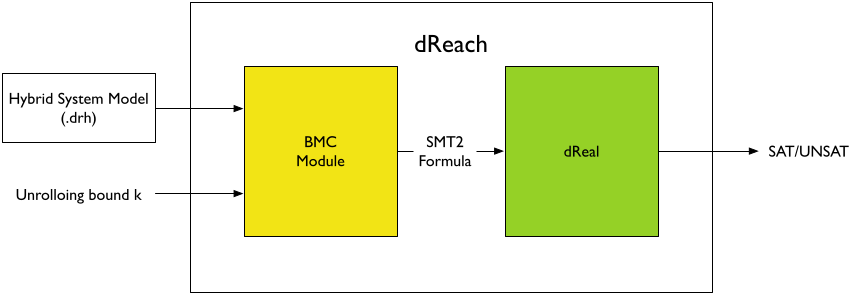
\includegraphics[width=\textwidth]{images/dReach}
  \caption{System Description of \dReach{}}
  \label{fig:system-description}
\end{figure}

Figure~\ref{fig:system-description} illustrates the architecture of
\dReach{}. We provide a domain-specific lanaguage to describe a hybrid
system and specify its safety properties. Given an input model,
specification, and unrolling bound $k$, \dReach{} reduces the
$\delta$-reachability problem to a $\delta$-decision problem of
formulas over the reals by providing a corresponding SMT encoding for
the problem. Then we answer the bounded reachability queries by using
our nonlinear SMT solver \dReal{}~\cite{DBLP:conf/cade/GaoKC13} to
solve the encoded problems.

\subsection{drh: a Language for Modeling and Specifying Hybrid Systems}

We define \texttt{drh}, a small language for describing hybrid systems
and specifying their initial and safety conditions. It consists of
five sections - macro definitions, variable declarations, mode
definitions, and initial condition, and goals.
\begin{align*}
  \textit{drh} := \ & \textit{macro-definition}^*\\
                  & \textit{variable-declaration}^+\\
                  & \textit{mode-definition}^+\\
                  & \textit{initial-condition}\\
                  & \textit{goal}^+
\end{align*}
In macro definitions, we allow users to define C-preprocessor macros
which can be used in following sections. Macros are expanded before
the other parts are processed.

A variable declaration has a form:
\[
\textit{variable-declaration} \ := \ \texttt{[}
                                     \textit{l}
                                     \texttt{,}
                                     \ \textit{u}
                                     \texttt{]}
                                     \ \textit{var}
                                     \texttt{;}
\]
and it declares a real variable $var$ whose domain is $[l, u] \in
\mathbb{IR}$. A special variable \textit{time} has to be delcared to
specify the time bound of bounded model checking.

A mode definition consists of mode id, mode invariant, flow, and jump.
\begin{align*}
  \textit{mode-definition} \ := & \ \texttt{\{}
                                    \texttt{mode} \ \textit{id}\texttt{;}\\
                           & \ \ \  \texttt{invt}:(\textit{formula} \texttt{;})^+\\
                           & \ \ \  \texttt{flow}:\textit{ode}^+\\
                           & \ \ \ \texttt{jump}:\textit{jump}^+ \texttt{\}}
\end{align*}
\textit{id} is a unique unsigned integer assigned to a mode. An
invariant is a conjuction of logic formulae which must hold in a mode.
A flow describes a continuous dynamics of a mode by providing a set of
ordinary differential equations (\textit{ode}s) which is a form of
``\texttt{d/dt[}\textit{x}\texttt{]=}\textit{exp}''. \textit{jump} is
a form of ``\textit{guard} \texttt{==>} \texttt{@}\textit{n}
\textit{reset}'' where \textit{guard} is a logic formula specifying a
condition to make a transition, $n$ is an id of target mode, and
\textit{reset} is a logic formula specifying the relationship between
old and new values.

\texttt{initial-condition} is of a form
``\texttt{@}\textit{mode-id} \textit{formula}\texttt{;}''
where \textit{mode-id} is an initial mode of a hybrid system and
\textit{formula} specifies the initial configuration of it.

\texttt{goal} shares the same syntactic structure,
``\texttt{@}\textit{mode-id} \textit{formula}\texttt{;}'' of
\textit{initial-condition} with a different interpretation. It poses a
reachability question: ``Is there a trajectory of a hybrid system
reaching \textit{mode-id} while satisfying the goal condition \textit{formula}?''.

\subsection{Encoding Bounded Reachability Problem}
\subsubsection{Encoding}
There are different encodings according to the requirements of the
solution. Out encoding formula is described in
\cite{gao2014delta}. The critical definitions that are related are
listed as follows:

\begin{definition}
Let $H$ be a hybrid automaton. We use $\unsafe = \{\unsafe_q:q\in Q\}$
in the state space of $H$. We can write $\llbracket \unsafe\rrbracket
= \bigcup_{q\in Q} \llbracket \unsafe_q \rrbracket\times \{q\}$.
\end{definition}

\begin{definition}
Let $Q = \{q_1,...,q_m\}$ be a set of modes. For any $q\in Q$, and
$i\in\mathbb{N}$, use $b_{q}^i$ to represent a Boolean variable. We
now define
$$\enforce_Q(q,i) = b^i_{q} \wedge \bigwedge_{p\in Q\setminus\{q\}}\neg b^{i}_{p}$$
$$\enforce_Q(q, q',i) = b^{i}_{q}\wedge \neg b^{i+1}_{q'} \wedge
\bigwedge_{p\in Q\setminus\{q\}} \neg b^i_{p} \wedge \bigwedge_{p'\in
  Q\setminus\{q'\}} \neg b^{i+1}_{p'}$$ We omit the subscript $Q$ when
the context is clear.
\end{definition}

\begin{definition}[$k$-Step Reachability, Invariant-Free Case]
Suppose $H$ is invariant-free, and $U$ a subset of its state space
represented by $\unsafe$. The $\lrf$-formula $\reach_{H,U}(k,M)$ is
defined as:
\begin{eqnarray*}
%\reach^{k,M}(H,U) &:=&
& &\exists^X \vec x_{0} \exists^X\vec x_{0}^t\cdots \exists^X \vec
  x_{k}\exists^X\vec x_{k}^t\exists^{[0,M]}t_0\cdots
  \exists^{[0,M]}t_k.\\ & &\bigvee_{q\in Q} \Big(\init_{q}(\vec
  x_{0})\wedge \flow_{q}(\vec x_{0}, \vec x_{0}^t, t_0)\wedge
  \enforce(q,0)\Big)\\%\wedge (b_{q_i}\wedge \bigwedge_{q\neq q_i}
  \neg b_{q}) \wedge & & \bigwedge_{i=0}^{k-1}\bigg( \bigvee_{q, q'\in
    Q} \Big(\jump_{q\rightarrow q'}(\vec x_{i}^t, \vec x_{i+1})\wedge
  \enforce(q,q',i)\\ & & \hspace{4.7cm}\wedge\flow_{q'}(\vec x_{i+1},
  \vec x_{i+1}^t, t_{i+1})\wedge \enforce(q',i+1)\Big)\bigg)\\ \wedge
  & & \bigvee_{q\in Q} \unsafe_q(\vec x_{k}^t).
\end{eqnarray*}
\end{definition}

%%% Local Variables:
%%% mode: latex
%%% TeX-master: "main"
%%% End:

\section{Example: Inelastic Bouncing Ball with Drag}
\begin{wrapfigure}{l}{0.5\textwidth}
  \centering
  \includegraphics[width=0.5 \textwidth]{images/bouncing_ball.pdf}
  \caption{Bouncing ball example}
  \label{fig:bouncing-ball}
\end{wrapfigure}


\begin{figure}
  \centering
  \begin{Verbatim}[fontfamily=courier, frame=single, framesep=1mm,
  numbers=left, fontsize=\scriptsize]
#define D 0.45
#define K 0.9
[0, 15] x;
[9.8] g;
[-18, 18] v;
[0, 3] time;
{
  mode 1;
  invt:
        (v <= 0);
        (x >= 0);
  flow:
        d/dt[x] = v;
        d/dt[v] = -g + (- D * v ^ 1);
  jump:
        (x = 0) ==> @2 (and (x' = x) (v' = - K * v));
}
{
  mode 2;
  invt:
        (v >= 0);
        (x >= 0);
  flow:
        d/dt[x] = v;
        d/dt[v] = -g + (- D * v ^ 1);
  jump:
        (v = 0) ==> @1 (and (x' = x) (v' = v));
}
init:
@1    (and (x >= 5) (v = 0));

goal:
@1    (and (x >= 0.45));
\end{Verbatim}
  \caption{Bouncing ball example}
  \label{fig:bouncing-ball}
\end{figure}

\begin{figure}
  \centering
  \begin{Verbatim}[fontfamily=courier, frame=single, framesep=1mm,
  numbers=left, fontsize=\scriptsize]
(set-logic QF_NRA_ODE)
(declare-fun x () Real)
(declare-fun v () Real)
(declare-fun x_0_0 () Real)
(declare-fun x_0_t () Real)
...
(declare-fun x_10_0 () Real)
(declare-fun x_10_t () Real)
(declare-fun v_0_0 () Real)
(declare-fun v_0_t () Real)
...
(declare-fun v_10_0 () Real)
(declare-fun v_10_t () Real)
(declare-fun time_0 () Real)
...
(declare-fun time_10 () Real)
(declare-fun mode_0 () Real)
...
(declare-fun mode_10 () Real)
(define-ode flow_1 ((= d/dt[x] v)
                    (= d/dt[v] (+ (- 0.0 9.8) (* -0.45 (^ v 1.0))))))
(define-ode flow_2 ((= d/dt[x] v)
                    (= d/dt[v] (+ (- 0.0 9.8) (* -0.45 (^ v 1.0))))))
(assert (<= 0.0 x_0_0))
(assert (<= x_0_0 15.0))
...
(assert (<= -18.0 v_10_t))
(assert (<= v_10_t 18.0))
(assert (<= 0.0 time_0))
(assert (<= time_0 3.0))
...
(assert (<= 0.0 time_10))
(assert (<= time_10 3.0))
...

(assert (and (and (= v_0_0 0.0) (>= x_0_0 5.0)) (= mode_0 1.0) (= [x_0_t v_0_t] (integral 0. time_0 [x_0_0 v_0_0] flow_1)) (= mode_0 1.0) (forall_t 1.0 [0.0 time_0] (<= v_0_t 0.0)) (<= v_0_t 0.0) (<= v_0_0 0.0) (forall_t 1.0 [0.0 time_0] (>= x_0_t 0.0)) (>= x_0_t 0.0) (>= x_0_0 0.0) (= mode_1 2.0) (= x_0_t 0.0) (= v_1_0 (* -0.9 v_0_t)) (= x_1_0 x_0_t) (= [x_1_t v_1_t] (integral 0. time_1 [x_1_0 v_1_0] flow_2)) (= mode_1 2.0) (forall_t 2.0 [0.0 time_1] (>= v_1_t 0.0)) (>= v_1_t 0.0) (>= v_1_0 0.0) (forall_t 2.0 [0.0 time_1] (>= x_1_t 0.0)) (>= x_1_t 0.0) (>= x_1_0 0.0) (= mode_2 1.0) (= v_1_t 0.0) (= v_2_0 v_1_t) (= x_2_0 x_1_t) (= [x_2_t v_2_t] (integral 0. time_2 [x_2_0 v_2_0] flow_1)) (= mode_2 1.0) (forall_t 1.0 [0.0 time_2] (<= v_2_t 0.0)) (<= v_2_t 0.0) (<= v_2_0 0.0) (forall_t 1.0 [0.0 time_2] (>= x_2_t 0.0)) (>= x_2_t 0.0) (>= x_2_0 0.0) (= mode_3 2.0) (= x_2_t 0.0) (= v_3_0 (* -0.9 v_2_t)) (= x_3_0 x_2_t) (= [x_3_t v_3_t] (integral 0. time_3 [x_3_0 v_3_0] flow_2)) (= mode_3 2.0) (forall_t 2.0 [0.0 time_3] (>= v_3_t 0.0)) (>= v_3_t 0.0) (>= v_3_0 0.0) (forall_t 2.0 [0.0 time_3] (>= x_3_t 0.0)) (>= x_3_t 0.0) (>= x_3_0 0.0) (= mode_4 1.0) (= v_3_t 0.0) (= v_4_0 v_3_t) (= x_4_0 x_3_t) (= [x_4_t v_4_t] (integral 0. time_4 [x_4_0 v_4_0] flow_1)) (= mode_4 1.0) (forall_t 1.0 [0.0 time_4] (<= v_4_t 0.0)) (<= v_4_t 0.0) (<= v_4_0 0.0) (forall_t 1.0 [0.0 time_4] (>= x_4_t 0.0)) (>= x_4_t 0.0) (>= x_4_0 0.0) (= mode_5 2.0) (= x_4_t 0.0) (= v_5_0 (* -0.9 v_4_t)) (= x_5_0 x_4_t) (= [x_5_t v_5_t] (integral 0. time_5 [x_5_0 v_5_0] flow_2)) (= mode_5 2.0) (forall_t 2.0 [0.0 time_5] (>= v_5_t 0.0)) (>= v_5_t 0.0) (>= v_5_0 0.0) (forall_t 2.0 [0.0 time_5] (>= x_5_t 0.0)) (>= x_5_t 0.0) (>= x_5_0 0.0) (= mode_6 1.0) (= v_5_t 0.0) (= v_6_0 v_5_t) (= x_6_0 x_5_t) (= [x_6_t v_6_t] (integral 0. time_6 [x_6_0 v_6_0] flow_1)) (= mode_6 1.0) (forall_t 1.0 [0.0 time_6] (<= v_6_t 0.0)) (<= v_6_t 0.0) (<= v_6_0 0.0) (forall_t 1.0 [0.0 time_6] (>= x_6_t 0.0)) (>= x_6_t 0.0) (>= x_6_0 0.0) (= mode_7 2.0) (= x_6_t 0.0) (= v_7_0 (* -0.9 v_6_t)) (= x_7_0 x_6_t) (= [x_7_t v_7_t] (integral 0. time_7 [x_7_0 v_7_0] flow_2)) (= mode_7 2.0) (forall_t 2.0 [0.0 time_7] (>= v_7_t 0.0)) (>= v_7_t 0.0) (>= v_7_0 0.0) (forall_t 2.0 [0.0 time_7] (>= x_7_t 0.0)) (>= x_7_t 0.0) (>= x_7_0 0.0) (= mode_8 1.0) (= v_7_t 0.0) (= v_8_0 v_7_t) (= x_8_0 x_7_t) (= [x_8_t v_8_t] (integral 0. time_8 [x_8_0 v_8_0] flow_1)) (= mode_8 1.0) (forall_t 1.0 [0.0 time_8] (<= v_8_t 0.0)) (<= v_8_t 0.0) (<= v_8_0 0.0) (forall_t 1.0 [0.0 time_8] (>= x_8_t 0.0)) (>= x_8_t 0.0) (>= x_8_0 0.0) (= mode_9 2.0) (= x_8_t 0.0) (= v_9_0 (* -0.9 v_8_t)) (= x_9_0 x_8_t) (= [x_9_t v_9_t] (integral 0. time_9 [x_9_0 v_9_0] flow_2)) (= mode_9 2.0) (forall_t 2.0 [0.0 time_9] (>= v_9_t 0.0)) (>= v_9_t 0.0) (>= v_9_0 0.0) (forall_t 2.0 [0.0 time_9] (>= x_9_t 0.0)) (>= x_9_t 0.0) (>= x_9_0 0.0) (= mode_10 1.0) (= v_9_t 0.0) (= v_10_0 v_9_t) (= x_10_0 x_9_t) (= [x_10_t v_10_t] (integral 0. time_10 [x_10_0 v_10_0] flow_1)) (= mode_10 1.0) (forall_t 1.0 [0.0 time_10] (<= v_10_t 0.0)) (<= v_10_t 0.0) (<= v_10_0 0.0) (forall_t 1.0 [0.0 time_10] (>= x_10_t 0.0)) (>= x_10_t 0.0) (>= x_10_0 0.0) (= mode_10 1.0) (>= x_10_t 0.45)))
(check-sat)
(exit)
\end{Verbatim}
  \caption{Bouncing ball example}
  \label{fig:bouncing-ball}
\end{figure}

%%% Local Variables:
%%% mode: latex
%%% TeX-master: "main"
%%% End:

\section{Using \dReach{}}\label{sec:using-dreach}

We now describe the input format and command line options of \dReach{}. 

\subsection{Input Format}\label{sec:input-format}

We now describe the input language for describing hybrid systems and
specifying reachability properties. It consists of five sections
- macro definitions, variable declarations, mode definitions, and
initial condition, and goals.
\begin{align*}
  \textit{drh} := \ & \textit{macro-definition}^*\\
                    & \textit{variable-declaration}^+\\
                    & \textit{mode-definition}^+\\
                    & \textit{initial-condition}\\
                    & \textit{goal}^+
\end{align*}
In macro definitions, it allows users to define macros in C
preprocessor (\texttt{cpp}) style which can be used in the following
sections. Note that macro expansions occur before the other parts are processed.

A variable declaration has a form:
\[
\textit{variable-declaration} \ := \ \texttt{[}
                                     \textit{l}
                                     \texttt{,}
                                     \ \textit{u}
                                     \texttt{]}
                                     \ \textit{var}
                                     \texttt{;}
\]
and it declares a real variable, $var$ and its domain $[l, u]$ which
is in Real interval $\mathbb{IR}$. It requires a special variable
declaration for \textit{time}, to specify the upperbound of time
duration in the analysis of bounded $\delta$-reachability.

A mode definition consists of mode id, mode invariant, flow, and jump.
\begin{align*}
  \textit{mode-definition} \ := & \ \texttt{\{}
                                    \texttt{mode} \ \textit{id}\texttt{;}\\
                           & \ \ \  \texttt{invt}:(\textit{formula} \texttt{;})^+\\
                           & \ \ \  \texttt{flow}:\textit{ode}^+\\
                           & \ \ \ \texttt{jump}:\textit{jump}^+ \texttt{\}}
\end{align*}
\textit{id} is a unique positive interger assigned to a mode. An
invariant is a conjuction of logic formulae which must always hold in
a mode. A flow describes a continuous dynamics of a mode by providing
a set of ordinary differential equations (\textit{ode}s) which is a
form of
``\texttt{d/dt[}\textit{x}\texttt{]=}\textit{exp}''. \textit{jump} is
a form of ``\textit{guard} \texttt{==>} \texttt{@}\textit{n}
\textit{reset}'' where \textit{guard} is a logic formula specifying a
condition to make a transition, $n$ denotes the target mode-id, and
\textit{reset} is a logic formula connecting the old and new values
for the transition.

\texttt{initial-condition} is of a form
``\texttt{@}\textit{mode-id} \textit{formula}\texttt{;}''
where \textit{mode-id} is an initial mode of a hybrid system and
\textit{formula} specifies the initial configuration of it.

\texttt{goal} shares the same syntactic structure,
``\texttt{@}\textit{mode-id} \textit{formula}\texttt{;}'' of
\textit{initial-condition} with a different interpretation. It poses a
reachability question: ``Is there a trajectory of a hybrid system
reaching \textit{mode-id} while satisfying the goal condition \textit{formula}?''.

\begin{figure}
  \centering
  \begin{Verbatim}[fontfamily=courier, frame=single, framesep=1mm,
  numbers=left, fontsize=\scriptsize]
#define D 0.45
#define K 0.9
[0, 15] x;
[9.8] g;
[-18, 18] v;
[0, 3] time;
{   mode 1;
    invt: (v <= 0);  (x >= 0);
    flow: d/dt[x] = v;
          d/dt[v] = -g - (D * v ^ 2);
    jump: (x = 0) ==> @2 (and (x' = x) (v' = - K * v)); }
 {  mode 2;
    invt: (v >= 0); (x >= 0);
    flow: d/dt[x] = v;
          d/dt[v] = -g + (D * v ^ 2);
    jump: (v = 0) ==> @1 (and (x' = x) (v' = v)); }
init: @1 (and (x >= 5) (v = 0));
goal: @1 (and (x >= 0.45));
\end{Verbatim}
\caption{An example of \drh{} format: Inelastic bouncing ball with air
  resistance. At lines 1 and 2, we define a drag coefficient $D = 0.45$
  and an elastic coefficient $K = 0.9$ using \texttt{\#define} macros.
  At lines 3 - 6, we declare variables $x, g, v,$ and $time$. At lines
  7 - 15 and 16 - 24, we define two modes -- the falling and the
  bouncing-back modes respectively. At lines 25 and 26, we specify
  that this hybrid system starts at mode 1 (\texttt{@1}) with initial
  condition satisfying $x \ge 5 \land v = 0$. At lines 28 and 29, it
  is asking whether we can have a trajectory ending at mode 1
  (\texttt{@1}) while the height of the ball is higher than $0.45$.}
\label{fig:bouncing-ball-drh}
\end{figure}

Figure~\ref{fig:bouncing-ball-drh} shows a canonical example of hybrid
systems, an inelastic bouncing ball with air resistance, in \drh{}
format.

%%% Local Variables:
%%% mode: latex
%%% TeX-master: "main"
%%% End:
\subsection{Command Line Options}
  \begin{Verbatim}[fontfamily=courier, frame=single, framesep=1mm, fontsize=\scriptsize]
usage: /home/soonhok/work/dreal/bin/dReach options <*.drh> <options to dReal>

dReach: Bounded Model Checking for for Nonlinear Hybrid Systems

OPTIONS:
   -k   unrolling steps  (default: 3)
   -b   use BMC heuristic with disjunctive path encoding
   -r   -b and filter unreachable modes from SMT encoding
   -e   -r and filter continuous variables from SMT encoding
   -d   disjunctive path encoding

EXAMPLE:

   dReach -k 10 bouncing_ball.drh --verbose --precision=0.001 --visualize

\end{Verbatim}

\begin{figure}
  \centering
  \includegraphics[width=\textwidth]{images/cardiac}
  \caption{Visualization of $\delta$-reachable trajectory for
    a cardiac-cell model.}
  \label{fig:viz}
\end{figure}


%%% Local Variables:
%%% mode: latex
%%% TeX-master: "main"
%%% End:

\input{application.tex}
\bibliographystyle{abbrv}
\bibliography{tau_tacas}
\end{document}
